\section{Анализ других алгоритмов, основанных на особых точках}

SIFT дескрипторы не лишены недостатков. Не все полученные точки и их дескрипторы будут отвечать предъявляемым требованиям. Естественно, это будет сказываться на дальнейшем решении задачи сопоставления изображений. В некоторых случаях решение может быть не найдено, даже если оно существует. Например, при поиске аффинных преобразований (или фундаментальной матрицы) по двум изображениям кирпичной стены может быть не найдено решения из-за того, что стена состоит из повторяющихся объектов (кирпичей), которые делают похожими между собой дескрипторы разных ключевых точек. Несмотря на это обстоятельство, данные дескрипторы хорошо работают во многих практически важных случаях. SIFT является наиболее математически обоснованным, но относительно медленным алгоритмом.

\subsection{Дескриптор SURF}

В 2008 был представлен ближайший конкурент SIFT дескриптора, \hyperref[itm:surf]{ SURF (Speeded up robust features) дескриптор [\ref{itm:surf}]}. В идейном смысле он похож на своего предшественника, но процедура описания окрестности особой точки несколько иная, поскольку в ней используются не гистограммы взвешенных градиентов, а отклики исходного изображения на \textit{вейвлеты Хаара} (\textbf{Haar wavelets}). Вейвлет — математическая функция, позволяющая анализировать различные частотные компоненты данных. Вейвлет Хаара — один из первых и наиболее простых вейвлетов, обладает компактным носителем, хорошо локализован в пространстве, но не является гладким.

На первом шаге получения дескриптора вокруг ключевой точки строится квадратная область, которую ориентируют по некоторому предпочтительному направлению. Затем область разделяется на квадратные сектора. В каждом из секторов в точках, принадлежащих регулярной сетке, вычисляются отклики на два вида вейвлетов — горизонтально и вертикально направленные. Отклики взвешиваются Гауссианом, суммируются по каждому сектору, и образуют первую часть дескриптора.

Вторая часть дескриптора SURF состоит из сумм модулей откликов. Это сделано для того, чтобы учитывать не только факт изменения яркости от точки к точке, но и сохранить информацию о направлении изменения. SURF-дескриптор имеет длину 64. Как и SIFT, SURF-дескриптор инвариантен к аддитивному изменению яркости. Инвариантность к мультипликативному изменению яркости достигается путем нормировки дескриптора. SURF является эвристическим, но и более быстрым, чем SIFT.

\subsection{Дескриптор BRIEF}

Чем меньше длина дескриптора, тем меньше памяти требуется для его хранения, и, соответственно, тем меньше времени тратится на сравнение их друг с другом. Эта характеристика играет очень значимую роль при обработке большого числа изображений большой размерности. К наиболее компактным относится дескриптор \hyperref[itm:brief]{ BRIEF (Binary Robust Independent Elementary Features) [\ref{itm:brief}]}. Для вычисления дескриптора в точке $p$ сравниваются значения яркости точек, расположенных в ее окрестности. При этом сравниваются значения яркости не всех точек со всеми, а анализируется лишь небольшое подмножество соседних пар точек, координаты которых распределены случайно (но одинаковым образом для каждой анализируемой точки $p$). Если яркость в точке $p_{i1}$ больше, чем яркость в точке $p_{i2}$, то $i$-я компонента дескриптора принимает значение $1$, в противном случае она становится равной нулю. Фрагмент, по которому вычисляются дескрипторы, предварительно сглаживается. BRIEF-дескрипторы чрезвычайно просты в вычислении, поскольку их значения равны результату сравнения двух чисел. Они также очень компактны, поскольку результат сравнения —- это число $0$ или $1$, то есть один бит.

В стандартной реализации для построения одного BRIEF-дескриптора требуется выполнить $256$ сравнений, что дает итоговую длину $32$ байта. Это очень мало, учитывая, что SIFT-дескриптор состоит из $128$ действительных чисел, то есть занимает как минимум $512$ байтов. Наконец, сравнение BRIEF-дескрипторов производится очень быстро, поскольку сводится к вычислению \textit{расстояния Хэмминга} между двумя последовательностями битов. Расстояние Хэмминга (\textbf{Hamming distance}) —- число позиций, в которых соответствующие символы двух слов одинаковой длины различны, -- вычисляется по формуле:

\begin{equation}
    d_{ij} = \sum_{k=1}^{p}|x_{ik} - x_{jk}|
\end{equation}

Эта элементарная операция выполняется чрезвычайно быстро на любом современном процессоре. Сами по себе дескрипторы BRIEF не инвариантны к повороту. Однако такой инвариантности можно добиться, если предварительно повернуть фрагмент вокруг ключевой точки на угол, соответствующий, например, доминирующему направлению градиента яркости, как это делается для дескрипторов SIFT и SURF. Точно так же можно достичь инвариантности к другим ракурсным искажениям.

\subsection{Дескриптор GLOH}

Дескриптор \hyperref[itm:gloh]{ GLOH (Gradient location-orientation histogram)} является модификацией SIFT-дескриптора и построен с целью повышения надежности \hyperref[itm:gloh]{[\ref{itm:gloh}]}. По факту вычисляется SIFT дескриптор, но используется полярная сетка разбиения окрестности на бины (рисунок \ref{fig:gloh}): 3 радиальных блока с радиусами 6, 11 и 15 пикселей и 8 секторов. В результате получается вектор, содержащий 272 компоненты, который проецируется в пространство размерности 128 посредством использования анализа главных компонент. Дескриптор GLOH наряду с SIFT является одним из самых точных методов.

\begin{figure}[h]
    \centering
    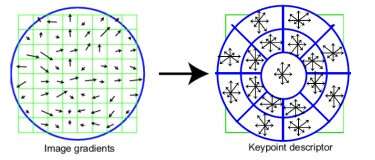
\includegraphics[width=0.8\textwidth]{gloh.jpg}
    \caption{Полярная сетка разбиения на бины}
    \label{fig:gloh}
\end{figure}

\subsection{Детектор FAST}

FAST (Features from accelerated segment test) -- алгоритм детекции ключевых точек.

Детектор считает пиксели в круге Брезенгема (находится с помощью алгоритма Брезенгема построения кривых 2-го порядка) радиуса $r$ вокруг точки кандидата. Если $n$ смежных пикселей ярче чем центр, по крайней мере, в $t$ раз или темнее центра, то пиксель в центре считается особенностью. Хотя $r$ в принципе, может принимать любое значение, чаще всего используется значение $r=3$, которому соответствует круг 16 пикселей окружности. Тесты показывают, что оптимальное значение $n=9$. Это значение $n$ наименьшее, при котором края не обнаруживаются.

\subsection{Дескриптор ORB}

ORB (Oriented FAST and rotated BRIEF) -- ещё один алгоритм основанный на детекторе ключевых точек FAST и бинарных дескрипторах BRIEF \hyperref[itm:orb]{[\ref{itm:orb}]}. Как следует из названия, ORB дополняет и улучшает алгоритмы, на которых был основан.

Алгоритм был предложен Ethan Rublee в 2010 году. Также как и BRIEF, ORB имеет размер 32 байта и для сравнения использует расстояния Хэмминга. После детектирования точек с помощью FAST-a ORB выделяет $N$ лучших точек, используя меру Харрисса. Далее ORB ориентирует найденные ключевые точки, что также отражено в его названии. Так как BRIEF плохо работает с поворотом, ORB исправляет это с помощью ориентации.
